\chapter{Experimentos}
\section{Protocolo de validación experimental}
Para el entrenamiento de los modelos se empleó la técnica de \textit{hold-out}, que consiste en dividir el conjunto de datos en dos subconjuntos principales: uno de entrenamiento y otro de test. A su vez, el conjunto de entrenamiento se subdivide para obtener un subconjunto adicional de validación. Durante el proceso de entrenamiento, el modelo es ajustado utilizando únicamente los datos del conjunto de entrenamiento, mientras que el conjunto de validación se utiliza para monitorizar el rendimiento del modelo en cada época, permitiendo detectar fenómenos como el sobreajuste y orientar procesos como el ajuste de hiperparámetros.

Una vez completado el entrenamiento, el modelo final se evalúa utilizando el conjunto de test, que se ha mantenido completamente aislado durante todo el proceso de ajuste, proporcionando así una estimación objetiva del rendimiento general del modelo sobre datos no vistos.

Como se ha descrito en la Sección \ref{section4:data_preparation} se utilizan tanto huesos izquierdos como derechos de los individuos. Dado que, desde el punto de vista anatómico, estos huesos presentan una alta similitud morfológica, realizar la partición del conjunto de datos a nivel de muestra podría derivar en una fuga de información (\textit{data leakage}). Para evitar este problema, la división del conjunto de datos se ha realizado a nivel de individuo: los huesos de un mismo sujeto se incluyen exclusivamente en uno de los subconjuntos (entrenamiento, validación o test) sin solapamiento entre ellos. De este modo, se garantiza que el modelo no memoriza las características particulares de un individuo, sino que generaliza adecuadamente aprendiendo patrones estructurales relevantes.

Este esquema de partición se ilustra en la Figura ???.
\section{Métricas}
Dado que se trata de un problema de clasificación, se emplea la función de pérdida de entropía cruzada (\textit{cross-entropy loss}) para ajustar los pesos y sesgos de las neuronas del modelo, tal como se explicó en la Sección \ref{section:DL}. Esta función se define de la siguiente forma:

\begin{equation}
L_{CE} = -\sum_i^n t_i \log(p_i)
\end{equation}

Donde $n$ es el número de clases, $t_i$ es la etiqueta verdadera (1 si la clase es la correcta, 0 en caso contrario) y $p_i$ es la probabilidad predicha para la $i$-ésima clase. Esta función penaliza con mayor intensidad aquellas predicciones que se alejan de la clase verdadera, incentivando al modelo a asignar una alta probabilidad a la clase correcta. Cuando la predicción es certera, el valor de la función tiende a cero; en cambio, si el modelo asigna baja probabilidad a la clase correcta, la función tiende a valores grandes positivos.

Adicionalmente, dado que el problema presenta un desbalance de clases, se han incorporado funciones de pérdida específicamente diseñadas para afrontar esta problemática. En particular, se han utilizado: la versión ponderada de la entropía cruzada (\textit{Weighted Cross Entropy}, WCE), la pérdida \textit{Focal} (FL) y la pérdida \textit{Class Balanced} (CB).

\begin{align}
    L_{WCE} &= -\sum_i^n \alpha_{i} t_i \log(p_i) \\
    L_{FL} &= -\sum_i^n (1-p_i)^{\gamma} t_i \log(p_i) \\
    L_{CB}(\textbf{p},y) &= \frac{1-\beta}{1-\beta^{n_{y}}} \mathcal{L}(\textbf{p},y)
\end{align}

En la WCE, el término $\alpha_i$ representa un peso específico para cada clase $i$, utilizado para reescalar la contribución de cada término de la pérdida. En este trabajo, se ha calculado $\alpha_i$ como el inverso de la frecuencia de la clase correspondiente, de modo que las clases menos representadas obtienen mayor peso, contrarrestando el sesgo del modelo hacia las clases mayoritarias.

Por su parte, la pérdida Focal (FL) extiende este enfoque mediante la incorporación del término $(1 - p_i)^\gamma$, donde $\gamma$ es un parámetro ajustable denominado factor de enfoque. Esta formulación reduce el impacto de las muestras correctamente clasificadas, es decir, aquellas con alta probabilidad en la clase verdadera y amplifica el efecto de aquellas muestras más difíciles de clasificar. Al hacerlo, se logra que el modelo se concentre en los casos menos representados.

La pérdida Class-Balanced (CB), en cambio, introduce una formulación más refinada del peso por clase, basada en el número efectivo de muestras. En lugar de utilizar directamente la frecuencia inversa de las clases, CB calcula un factor de corrección con el parámetro $\beta$ que refleja mejor la cantidad de información aportada por cada clase. Esta técnica puede aplicarse como un prefactor sobre diferentes funciones de pérdida $\mathcal{L}(\mathbf{p}, y)$, siendo compatible tanto con WCE como con FL, entre otras.

Aunque estas funciones de pérdida son fundamentales para guiar el proceso de entrenamiento y seleccionar el mejor modelo, no ofrecen información directa sobre el rendimiento del clasificador en términos de aciertos y errores. Para ello, se emplea la métrica de \textit{accuracy}, que cuantifica la proporción de muestras clasificadas correctamente. Esta métrica se define como:

\begin{equation}
\text{Accuracy} = \frac{TP + TN}{TP + TN + FP + FN}
\end{equation}

donde $TP$ (verdaderos positivos) y $TN$ (verdaderos negativos) representan las predicciones correctas, mientras que $FP$ (falsos positivos) y $FN$ (falsos negativos) corresponden a errores de clasificación.

A pesar de su carácter intuitivo y simplicidad, el \textit{accuracy} puede inducir a interpretaciones erróneas cuando se trabaja con conjuntos de datos desbalanceados, ya que no distingue entre los distintos tipos de errores y puede sobreestimar el rendimiento del modelo en clases mayoritarias.

Por ello, la métrica que se utilizará como criterio principal para emitir un veredicto final sobre la calidad del aprendizaje es el valor F1, definido como:

\begin{equation}
    \text{F1} = 2 \cdot \frac{\text{Precision} \cdot \text{Recall}}{\text{Precision} + \text{Recall}}
    \end{equation}

donde las métricas de \textit{precision} y \textit{recall}, en el contexto binario, se definen como:
\begin{align}
    \text{Precision} &= \frac{TP}{TP + FP} \\
    \text{Recall} &= \frac{TP}{TP + FN}
\end{align}

La \textit{precision} indica qué proporción de las predicciones positivas realizadas por el modelo son correctas, mientras que \textit{recall} mide la proporción de muestras realmente positivas que fueron correctamente identificadas. Estas métricas permiten detectar posibles sesgos en el comportamiento del modelo, tales como una mayor propensión a cometer falsos positivos o falsos negativos.

Dado que en este proyecto se busca una clasificación lo más equilibrada posible entre clases, se opta por utilizar la métrica F1, que representa un balance armónico entre \textit{precision} y \textit{recall}. En particular, se utiliza la media macro del F1, la cual considera por igual todas las clases, sin ponderarlas según su frecuencia. Este enfoque es especialmente adecuado en contextos con desbalance de clases, ya que asegura que cada clase contribuya equitativamente a la métrica. Su cálculo se basa en las versiones multiclase de \textit{precision} y \textit{recall}, definidas como:

\begin{align}
    \text{Precision}_{\text{Macro}} &= \frac{\text{Precision}_{\text{Clase A}}+\text{Precision}_{\text{Clase B}}+\dots+\text{Precision}_{\text{Clase N}}}{N} \\
    \text{Recall}_{\text{Macro}} &= \frac{\text{Recall}_{\text{Clase A}}+\text{Recall}_{\text{Clase B}}+\dots+\text{Recall}_{\text{Clase N}}}{N}
\end{align}

Durante el proceso de ajuste de hiperparámetros y búsqueda automática de arquitectura (NAS), llevado a cabo mediante Optuna, como se detalla en la Sección \ref{section4:nas}, fue necesario definir una función objetivo (\textit{fitness}) que guiara la optimización. Dada la naturaleza desbalanceada del problema, se eligió la métrica F1 macro como base para esta función. El valor de fitness se define como:

\begin{equation}
    \text{Fitness} = \text{F1}_{\text{Validación}} \cdot (1 - | \text{F1}_{\text{Validación}} -  \text{F1}_{\text{Entrenamiento}}|)
\end{equation}

La intuición detrás de esta formulación es doble: por un lado, se favorecen modelos con un alto rendimiento en el conjunto de validación, y por otro, se penaliza la discrepancia entre el rendimiento en entrenamiento y validación, lo cual es indicativo de sobreajuste. De este modo, se priorizan aquellos modelos que generalizan bien y no simplemente memorizan los datos de entrenamiento.

Por último, se incorpora una métrica adicional, la distancia de Hausdorff, que no evalúa directamente el rendimiento del modelo, sino la calidad geométrica de las mallas poligonales. Formalmente, esta distancia se define como:

\begin{equation}
d_H = \max\left\{\sup_{x\in X} \inf_{y \in Y} d(x,y), \sup_{y\in Y} \inf_{x \in X} d(x,y) \right\}
\end{equation}

donde $X$ e $Y$ son subconjuntos del espacio métrico, y $d(x,y)$ representa la distancia entre los puntos $x$ e $y$. En el contexto de las mallas 3D \cite{cignoni1998metro}, se evalúa esta métrica entre triángulos de dos mallas distintas, permitiendo cuantificar la similitud o diferencia entre sus superficies. Para su cálculo se ha empleado PyMeshLab, el cual proporciona tanto la distancia máxima como la distancia media entre las superficies comparadas, expresadas en unidades absolutas (metros, centímetros, etc.) o como un porcentaje relativo.

\section{Análisis de pérdida de calidad de mallas 3D al reducir el número de triángulos}
\label{section5:experiment_edge_collapse}
Como se ha explicado en la Sección \ref{section4:methods}, el método ExMeshCNN requiere que todas las mallas tengan un número idéntico de caras triangulares para poder procesarlas correctamente. Sin embargo, como se mencionó en la Sección \ref{section4:data_preparation}, las mallas del conjunto de datos original presentan un número variable de triángulos, y además, muchas de ellas contienen una cantidad excesiva de caras que supera las capacidades del hardware disponible.

Por este motivo, es importante evaluar el impacto que tiene la reducción del número de triángulos sobre la calidad topológica de las mallas. En particular, se busca responder la siguiente pregunta: ¿en qué medida se ve afectada la topología de una malla al aplicar técnicas de simplificación por colapso de aristas?

\begin{figure}[h]
    \centering
    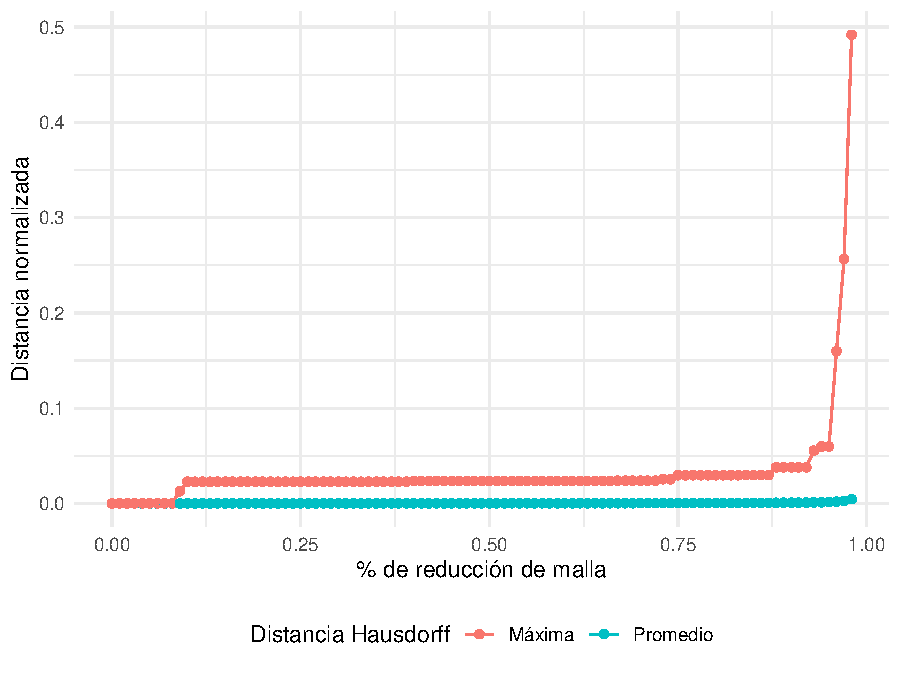
\includegraphics[width=\linewidth]{figures/4_experiments/mesh_redux_study.pdf}
    \caption[Estudio de reducción de mallas]{Distancia Hausdorff normalizada entre las mallas originales y sus versiones reducidas a distintos porcentajes del número original de triángulos. En este experimento, la reducción se realizó en incrementos del 1\%.}
    \label{fig5:redux_study}
\end{figure}

Para abordar esta cuestión, se diseñó un experimento en el que se toma una malla original y se generan versiones reducidas conservando distintas proporciones del número de triángulos originales (por ejemplo, 75\%, 50\%, 25\%, etc.). Posteriormente, estas versiones simplificadas se comparan con la malla original utilizando la distancia de Hausdorff, con el fin de cuantificar la desviación de la superficie resultante respecto de la original.

En la Figura \ref{fig5:redux_study} se presenta la evolución de la distancia Hausdorff normalizada al reducir progresivamente el número de triángulos de las mallas. Esta distancia ha sido normalizada respecto a la diagonal de la \textit{bounding box} de cada malla original, lo que permite comparar directamente las deformaciones relativas entre mallas de diferentes tamaños y complejidades geométricas. Además, esta normalización facilita el cálculo de promedios globales entre las distintas muestras evaluadas.

Como puede observarse, hasta una reducción del 75\% del número de triángulos, el error promedio permanece esencialmente cercano a cero, lo que sugiere una alta fidelidad en la preservación de la geometría original. Durante este mismo rango, el error máximo crece lentamente, manteniéndose al rededor del 0.2\% de variación con respecto a la malla original. Es únicamente a partir de reducciones superiores al 90\% cuando se observa un incremento más pronunciado del error máximo, aunque el error promedio aún se mantiene relativamente controlado.

Estos resultados apuntan a que es posible aplicar reducciones agresivas en la cantidad de triángulos sin comprometer significativamente la calidad topológica de las mallas. En consecuencia, se valida la viabilidad de utilizar versiones simplificadas de las mallas para el entrenamiento por medio de ExMeshCNN.

\section{Experimentos con etiqueta única}
Una vez validado que es factible utilizar versiones reducidas de las mallas sin pérdida significativa de información, y habiendo preparado los datos para su uso con el modelo ExMeshCNN, tal como se describe en la Sección \ref{section4:data_preparation}, se procedió a diseñar la estrategia para la generación automática de arquitecturas, explicada en profundidad en la Sección \ref{section4:nas}.

En esta fase, se llevaron a cabo los denominados experimentos de etiqueta única, donde se entrena un modelo independiente para cada una de las características de Todd, sin considerar la influencia de las demás características.

Por cada característica, se realizaron 6 ejecuciones distintas resultantes de las combinaciones de los siguientes parámetros:

\begin{itemize}
\item \textbf{Resolución de la malla}: 100,000 (o 100K); 50,000 (50K) y 25,000 (25K) triángulos.
\item \textbf{Tipo de malla}: Malla completa (Full) o malla recortada (Cut).
\end{itemize}

Cada ejecución implicó la realización de 200 entrenamientos utilizando Optuna para la búsqueda de arquitectura neuronal y optimización de hiperparámetros, con el fin de obtener el modelo más adecuado para predecir cada característica de forma individual.

Dado que se tienen 9 características de Todd, y para cada una se ejecutaron 6 combinaciones con 200 entrenamientos, el número total de entrenamientos realizados asciende a $9\times6\times200=10,800$ entrenamientos totales.

Esto equivale a $1,800$ entrenamientos por característica, lo que refleja el alto grado de exploración llevado a cabo para asegurar un modelo óptimo en cada caso.

\begin{table}[h]
    \centering
    \begin{tabular}{|c|c|c|c|c|}
    \hline
    \rowcolor[HTML]{D33333} 
    {\color[HTML]{FFFFFF} Característica} & {\color[HTML]{FFFFFF} Test Accuracy} & {\color[HTML]{FFFFFF} Test F1} & {\color[HTML]{FFFFFF} Resolución} & {\color[HTML]{FFFFFF} Tipo} \\ \hline
    AF & 0.6546 & 0.4729 & 50K & Cut \\
    BN & 0.9158 & 0.6916 & 25K & Cut \\
    DM & 0.7333 & 0.6261 & 25K & Cut \\
    DP & 0.8827 & 0.7113 & 25K & Cut \\
    IP & 0.7113 & 0.5410 & 100K & Cut \\
    LSE & 0.9800 & 0.9232 & 100K & Full \\
    USE & 0.9797 & 0.8281 & 25K & Cut \\
    VB & 0.5202 & 0.5275 & 50K & Cut \\
    VM & 0.6954 & 0.6747 & 50K & Cut \\ \hline
    \end{tabular}
    \caption{Cuadro resumen de los mejores modelos obtenidos para cada característica}
    \label{table5:single_tag__results}
\end{table}

Como se puede observar en la Tabla \ref{table5:single_tag__results}, existe una considerable variabilidad en los valores obtenidos para la métrica F1 al evaluar cada modelo sobre el conjunto de test. No obstante, en la mayoría de los casos se han alcanzado resultados satisfactorios, con valores de F1 superiores a 0.5 en todos los modelos, además de un \textit{accuracy} generalmente elevado.

Es particularmente destacable el desempeño de las características LSE y USE, que han alcanzado resultados sobresalientes a pesar de presentar un alto grado de desbalance en las etiquetas, como se evidenció en el EDA (Sección \ref{section4:data_eda}). Esto sugiere la presencia de patrones bien definidos en la superficie ósea que han sido correctamente capturados por los modelos, permitiendo lograr simultáneamente un \textit{accuracy} muy alto y valores de F1 igualmente notables. En contraste, otras dos características también altamente desbalanceadas, como BN y DP, si bien obtuvieron buenos resultados, se encuentran dentro del rango de desempeño general de las demás características más balanceadas, lo que refuerza la hipótesis de que LSE y USE presentan una topología más informativa o distinguible para las redes.

Por otro lado, la característica VB, que presenta la distribución más balanceada de etiquetas, fue la que obtuvo el rendimiento más bajo tanto en términos de \textit{accuracy} como de F1. Esto podría indicar que, pese a un buen balance, los patrones topológicos asociados a esta característica son más sutiles o complejos de identificar, lo cual plantea un reto adicional para el modelo.

El resto de las características muestran un comportamiento relativamente uniforme, sin una clara correlación entre el grado de desbalance y el rendimiento del modelo, lo que a su vez sugiere que el enfoque de entrenamiento adoptado ha sido eficaz para extraer información relevante incluso en escenarios con clases altamente desbalanceadas y una cantidad limitada de datos.

Un aspecto adicional a destacar es el impacto del tipo de malla utilizada. Exceptuando el modelo de LSE, todos los demás alcanzaron mejores resultados al emplear las versiones recortadas de las mallas. Este comportamiento respalda la hipótesis de que eliminar estructuras óseas irrelevantes (según la práctica de los expertos) permite concentrar el poder de representación del modelo en la zona de interés, reduciendo el ruido y facilitando la identificación de patrones significativos. En el caso de LSE, sin embargo, las mallas completas resultaron más beneficiosas, lo cual podría implicar que la información relevante para esta característica se encuentra distribuida también fuera de la región habitualmente considerada como de interés.

Respecto a la resolución, se observa que los mejores resultados, en general, se obtuvieron con la resolución más baja de 25K triángulos, seguida de 50K, y solo dos modelos alcanzaron su mejor desempeño con 100K triángulos. Esta observación concuerda con lo reportado por los autores de ExMeshCNN \cite{kim_exmeshcnn_2022}, donde también se encontró que las mallas de menor resolución producían mejores resultados. Se teoriza que esto se debe a que, al aumentar la resolución, la operación de \textit{global average pooling} que conecta las capas convolucionales con las totalmente conectadas podría estar diluyendo información crítica al comprimir un mayor número de triángulos en una única representación.

Sin embargo, las características LSE e IP constituyen una excepción a esta tendencia: en ambos casos, la mayor resolución permitió obtener un mejor rendimiento, lo que indica que para estas características el mayor nivel de detalle en la superficie ósea proporciona una ventaja en el aprendizaje del modelo.

Cabe resaltar que, si bien esta tabla resumen permite una visión general del rendimiento de los modelos, no ofrece por sí sola un panorama completo. Por esta razón, en las siguientes subsecciones se llevará a cabo un análisis detallado de los resultados obtenidos para cada una de las características de Todd.

\subsection{AF}



\subsection{BN}
\subsection{DM}
\subsection{DP}
\subsection{IP}
\subsection{LSE}
\subsection{USE}
\subsection{VB}
\subsection{VM}

\section{Experimentos multietiqueta}

\subsection{AF}
\subsection{BN}
\subsection{DM}
\subsection{DP}
\subsection{IP}
\subsection{LSE}
\subsection{USE}
\subsection{VB}
\subsection{VM}

\section{Interpretación con Grad-CAM}

\subsection{AF}
\subsection{BN}
\subsection{DM}
\subsection{DP}
\subsection{IP}
\subsection{LSE}
\subsection{USE}
\subsection{VB}
\subsection{VM}
